%%%%%%%%%%%%%%%%%%%%%%%%%%%%%%%%%%%%%%%%%%%%%%
%                insertmeeting
% 1) Title (something creative & funny?)
% 2) Date (MM/DD/YYYY)
% 3) Location (ex. Hagerty High School)
% 4) People/Committees Present 
% 5) Picture 
% 6) Start Time & Stop Time (ex. 12:30AM to 4:30PM)
%%%%%%%%%%%%%%%%%%%%%%%%%%%%%%%%%%%%%%%%%%%%%%
\insertmeeting 
	{Subsystems} 
	{10/04/21} 
	{Hagerty High School}
	{Anouska, Clayton, Jensen, Nathan, Ritam, Rose, Samantha, Lilly}
	{Images/RobotPics/robot.jpg}
	{2:30 - 4:30}
	
\hhscommittee{Software}
\noindent\hfil\rule{\textwidth}{.4pt}\hfil
\subsubsection*{Goals}
\begin{itemize}
    \item Start working on subsystems  

\end{itemize} 

\noindent\hfil\rule{\textwidth}{.4pt}\hfil

\subsubsection*{Accomplishments}
Today, we started to work on our subsystems. We always like to utilize object-oriented programming because it is more structured and allows for us to learn the ways of how adult programmers write code. One of the classes we created today was the Carousel class which was just made to test a 20:1 Rev Motor with a 4 inch wheel. We found that the power was a little too fast and decided that next meeting we would try to limit the power. We believed that a 25:1 rev motor would be just the perfect speed to go quick and be able to get all the ducks with accuracy. We did some quick math and found that the RPM needed to go would 1 * (20/25) which is just 0.8. We plan to test this at our next meeting.


\begin{figure}[htp]
\centering
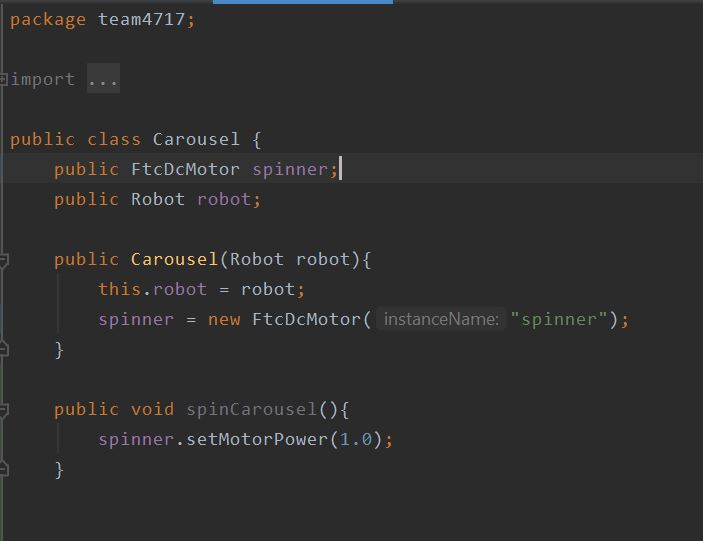
\includegraphics[width=0.95\textwidth, angle=0]{Meetings/October/10-04-21/Capture - Ritam R.JPG}
\caption{Our carousel class}
\label{fig:pic1}
\end{figure}


\whatsnext{
\begin{itemize}
    \item Test a lower power
\end{itemize} 
}

